The Lock-in+PID application is currently used in the experiment to maintain the intensity of the laser beam that probes the Rydberg atoms in the cavity. The application was first created by Marcelo Alejandro Luda in the context of a Physics PhD career at the Universidad de Buenos Aires \cite{lipid}. It includes an oscilloscope application (adapted from the default one that comes with the Red Pitaya) and a lock-in amplifier. Figure \ref{fig:ch2_li_pid} presents a screenshot of the application interface, showing the two input signal data collected by the oscilloscope, as well as various other configuration panels. The application allows the user to capture and plot a desired length of signal data that can be easily saved to different file types for further studies. Therefore, we hoped to adapt the oscilloscope of the Lock-in+PID to satisfy the experimental requirements predicted in Equation \eqref{eq:rp_memory}.

\begin{figure}[ht]
    \centering
    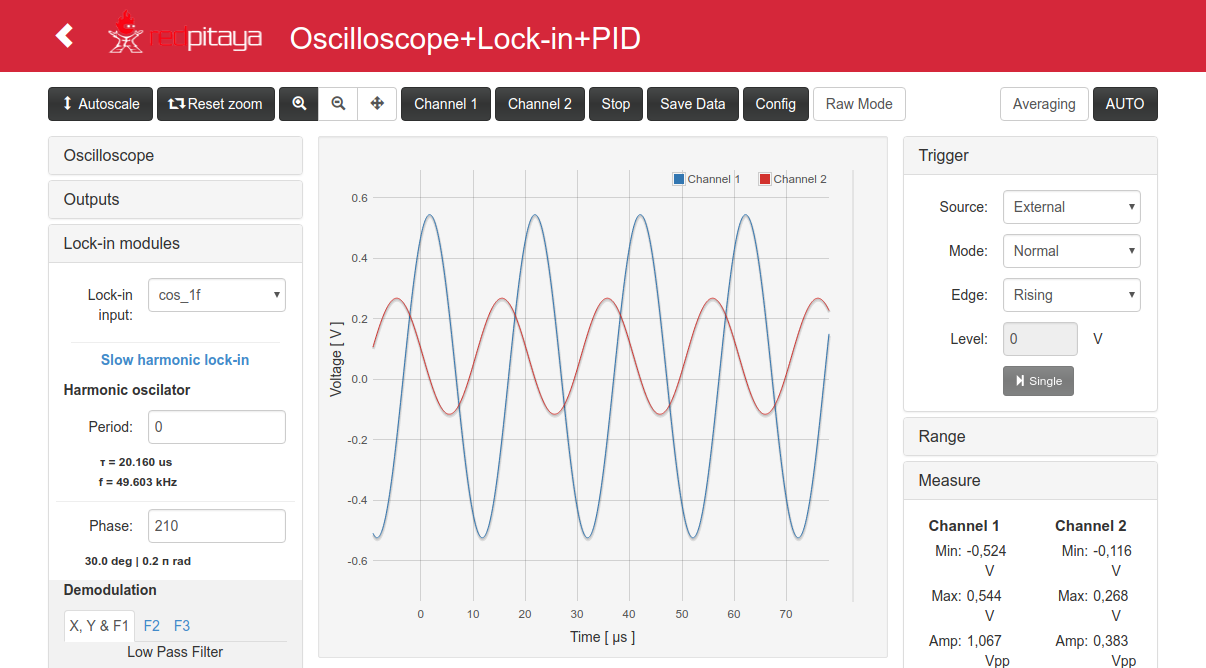
\includegraphics[width=0.8\columnwidth]{images/chapter_2/2_li_pid/li_pid.png}
    \caption{Screenshot of the Lock-in+PID application interface.}
    \label{fig:ch2_li_pid}
\end{figure}

%%%%%%%%%%%%%%%%%%%%%%%%%%%%%%%%%%%%%%%%%%%%%%%%%%%%%%%%%%%%%%%%%%%%%%%%%%%%%%%%

\paragraph{Hardware Modification}

By default, the oscilloscope application samples data at the maximum rate of 125 MHz, and occupies 1 IP (intellectual property) core, starting from system address \texttt{0x40100000} and ending at \texttt{0x401FFFFF} \cite{rp}. This corresponds to 16$^5$ bytes = 1,048,576 bytes $\sim$ 1 MB of memory space. So the objective was then to understand how the oscilloscope of the Lock-in+PID application captures, stores, and reads input data to and from the RAM, so that we can accordingly modify the memory allocation and storage for our experimental needs.

To begin, I explored the Verilog code that configures the oscilloscope hardware, which is comprised of the following main parts:
\begin{itemize}\setlength{\itemsep}{1pt}
    \item \textbf{Trigger:} configures the trigger for the ADC
    \item \textbf{ADC input data filtering:} the input signal data captured and converted by the ADC are filtered based on configuration coefficients
    \item \textbf{Input data decimation:} the rate of data captured is reduced while maintaining the essential information
    \item \textbf{Buffer RAM:} writing to and reading from the buffer RAM where the data captured by the ADC are temporarily stored
    \item \textbf{AXI (Advanced eXtensible Interface) connection:} protocol that enables efficient communication between different components on the Red Pitaya
    \item \textbf{System bus connection:} assigns values for various system address variables and stores input data read from the buffer RAM to the designated addresses on the allocated IP core
\end{itemize}

The Verilog code of the oscilloscope reveals that $2^{14} = 16,384$ samples of ADC data per input channel are stored into the appropriate IP core memory space. By default, each sample takes up only 14 bits, but is stored in a 32-bit (4-byte) chunk of system memory, with the upper 18 bits being insignificant. This is because the Red Pitaya transfers system memory data in 4-byte chunks. Correspondingly, 65,536 bytes of data are saved to system memory at once by the oscilloscope hardware per input channel, with channel A data starting from system address \texttt{0x40110000} and channel B data starting from system address \texttt{0x40120000}. Given that 1 MB of memory space is reserved for the oscilloscope application, we are then able to exploit the unused space starting from system address \texttt{0x40130000} for our purposes.

To extend the amount of data saved to system memory at once, I modified the Verilog code in the \textbf{system bus connection} section by extending the system address into the unused memory addresses and storing the 14 significant bits of channel B sample into the unused bits of the 4-byte chunk for each channel A sample. This allowed an 8-fold increase in captured data storage into the system memory per channel, corresponding to 131,072 samples or roughly 0.25 MB per channel, meeting our predicted experimental needs described by Equation \eqref{eq:rp_memory} exactly.

%%%%%%%%%%%%%%%%%%%%%%%%%%%%%%%%%%%%%%%%%%%%%%%%%%%%%%%%%%%%%%%%%%%%%%%%%%%%%%%%

\paragraph{Software Modification}

Subsequently, it was necessary to explore and modify accordingly the software code written in C that reads and processes the ADC input data stored in the system RAM for the front-end oscilloscope web application. This included updating the extended memory addresses and sample length for data reading, and extracting appropriately each sample for channel A and B now stored side-by-side in 4-byte chunks.

\begin{figure}[ht]
    \centering
    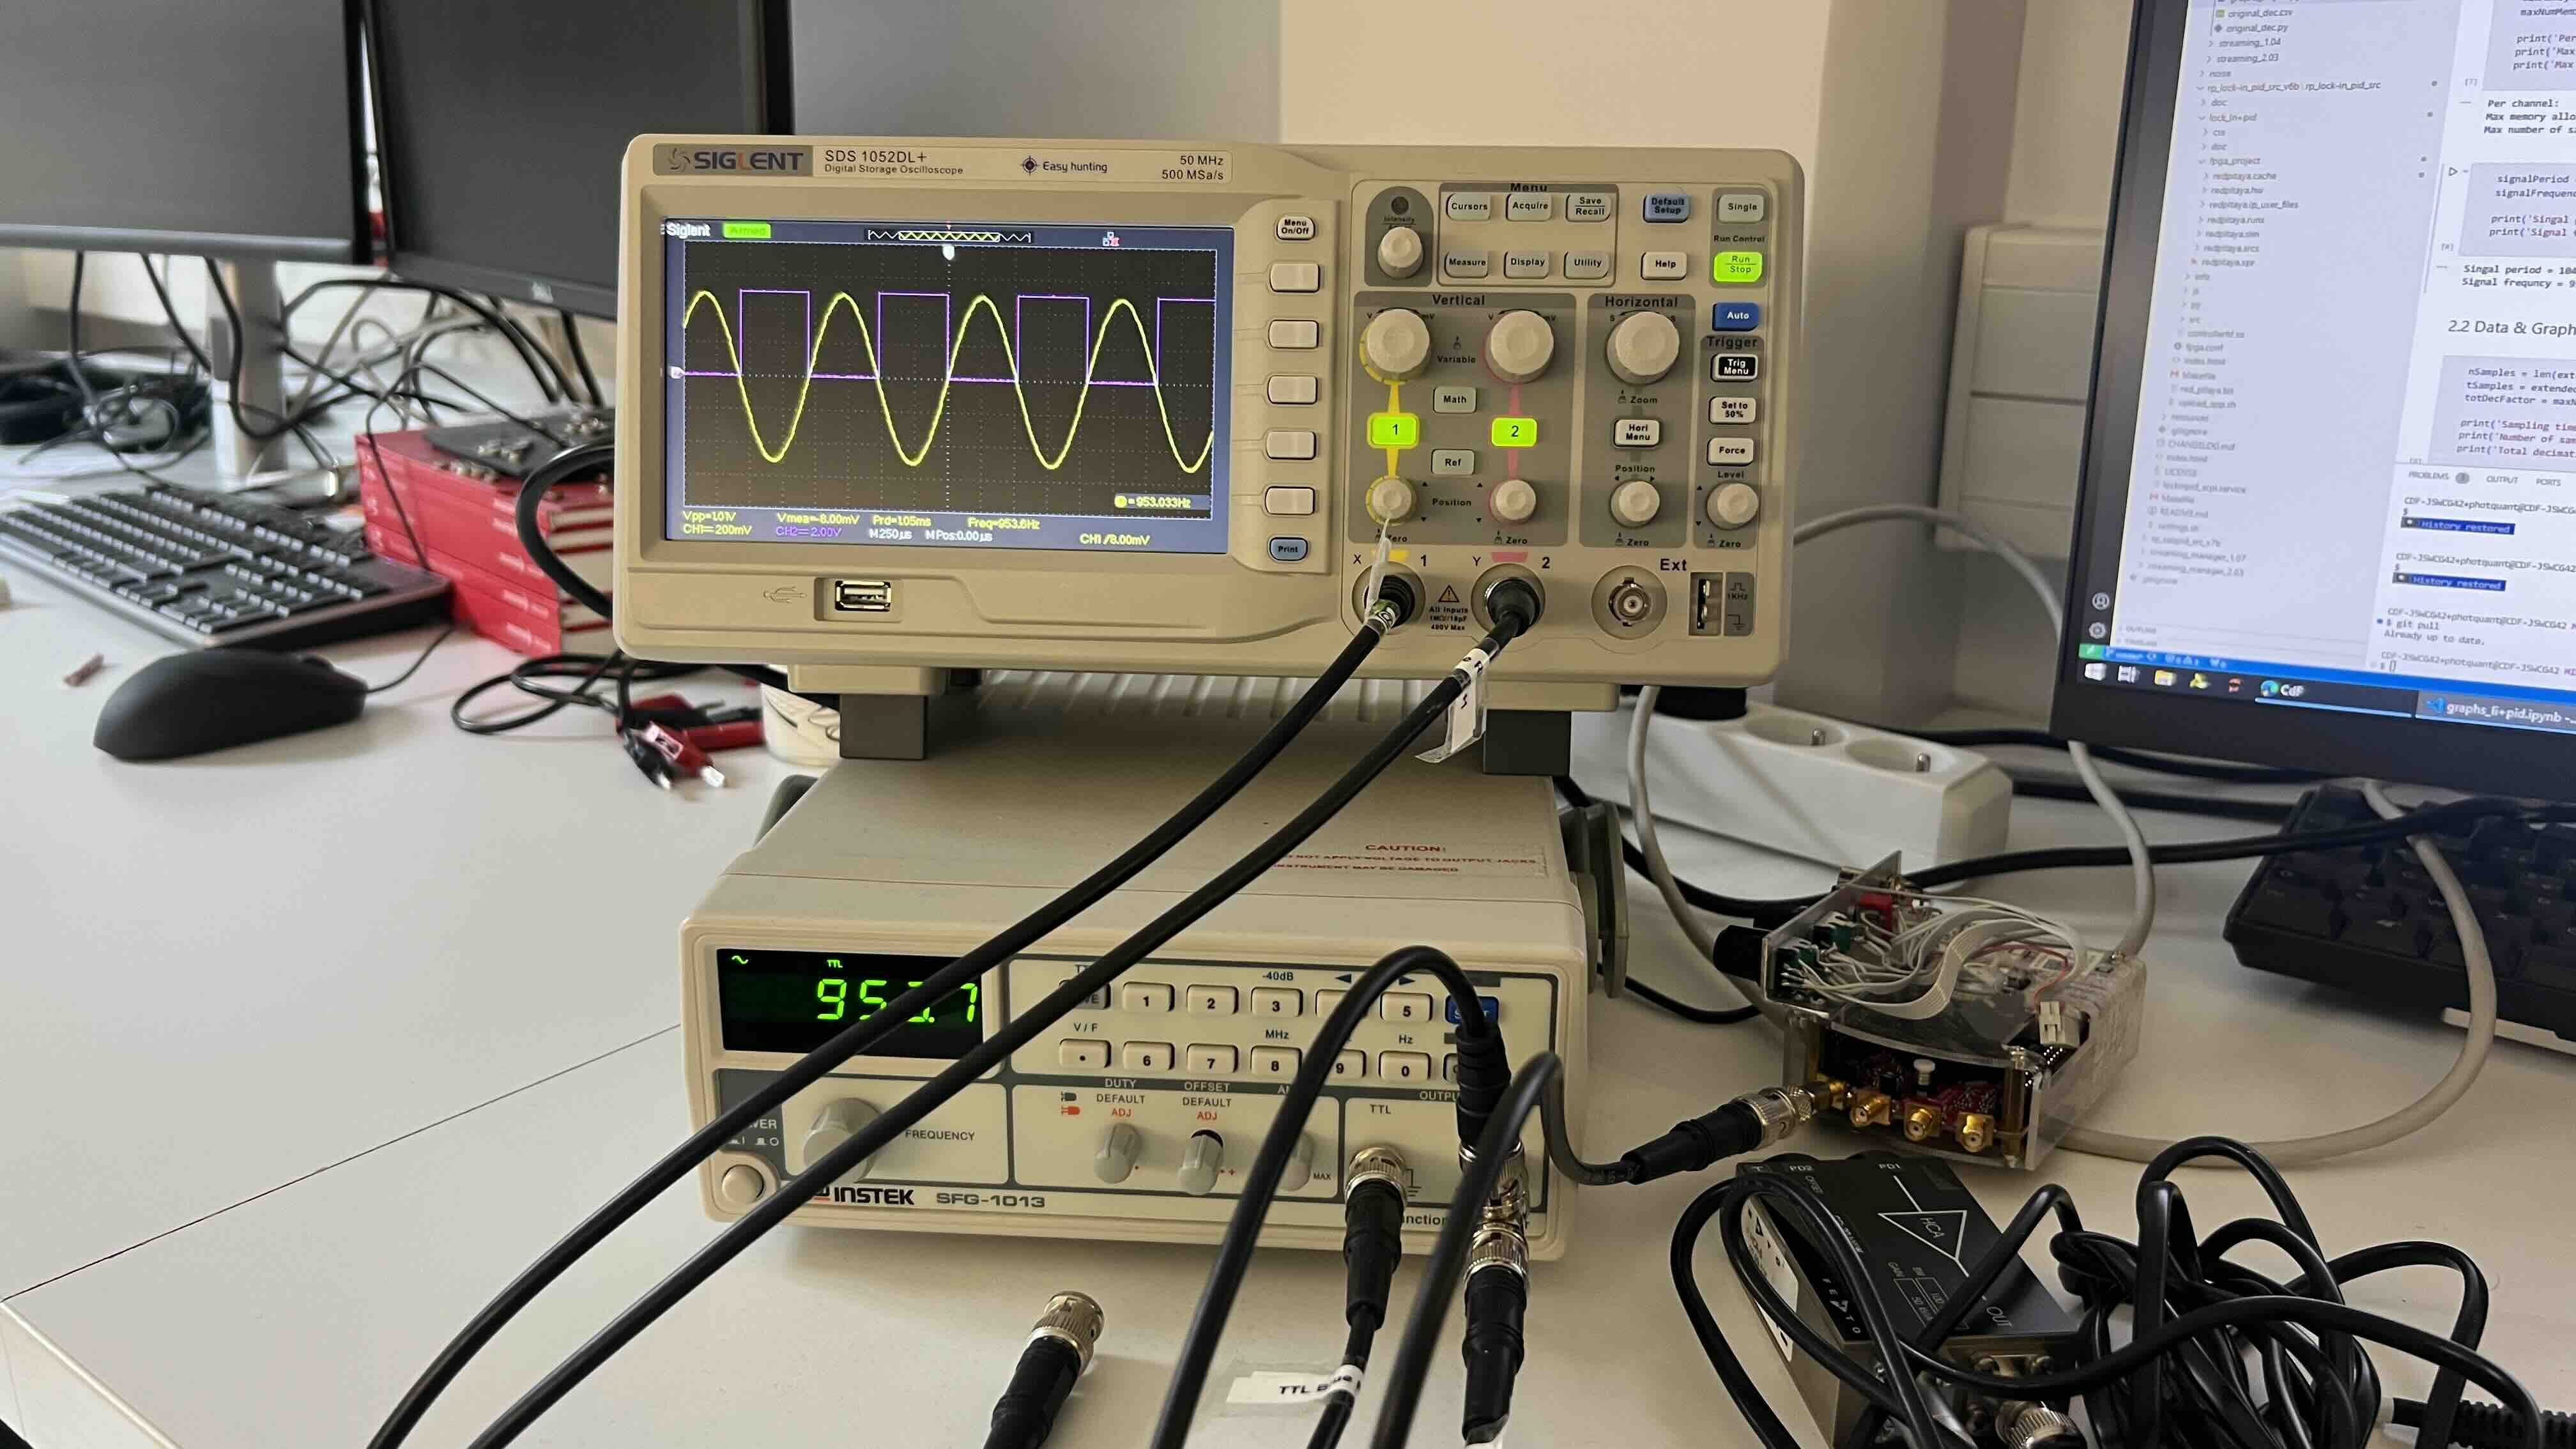
\includegraphics[width=0.75\columnwidth]{images/chapter_2/signal_generator.jpeg}
    \caption{Input signal generator (bottom) for conducting tests for the Red Pitaya and external oscilloscope (top) to visualize and confirm the configured input signals.}
    \label{fig:ch2_signal_generator}
\end{figure}

%%%%%%%%%%%%%%%%%%%%%%%%%%%%%%%%%%%%%%%%%%%%%%%%%%%%%%%%%%%%%%%%%%%%%%%%%%%%%%%%

\paragraph{Tests}

A simple method to test whether the memory was successfully extended is to monitor the memory addresses that were previously unused consecutively and observe the value stored. For example, executing in the Red Pitaya kernal \textbf{\texttt{monitor 0x40130000}} multiple times by hand, and reading the value stored at this memory address that's not used by default. If the memory was not extended correctly, the output values will only fluctuate slightly due to noise. If the memory was extended correctly, the output values will fluctuate by a large amount because varying sample points of the input signal will be stored at that address. This method is by no means comprehensive but is sufficient as a quick check.

Additionally, we configure the input signal at a frequency such that sampling exactly 1 period of the signal will fill up the entire memory space dedicated to a single channel, i.e.
\begin{equation}\label{eq:f_full}
    f_\text{full} = \frac{\text{sampling rate}}{\text{max number of samples storable in memory at once}}\ .
\end{equation}
This allows a quick visual verification that the test acquisitions were collecting data in an expected manner, that is, exactly one period of the waveform. Using the original oscilloscope application as an example, which stores up to 16,384 samples at once, at a sampling rate of 125 MHz, this corresponds to a $f_\text{full} = 7629$ Hz and a period of $T_\text{full} = 131\ \mu$s. And for the oscilloscope application with 8-fold extended memory space, $f_\text{full} = 954$ Hz and $T_\text{full} = 1049\ \mu$s.

Figure \ref{fig:ch2_signal_generator} shows the setup of such a memory test with the Red Pitaya, where a sinusoidal analog signal is created by a signal generator. The signal is connected to an external oscilloscope for monitoring and to the Red Pitaya's input channel A.

%%%%%%%%%%%%%%%%%%%%%%%%%%%%%%%%%%%%%%%%%%%%%%%%%%%%%%%%%%%%%%%%%%%%%%%%%%%%%%%%

\paragraph{Results}

With the \textbf{\texttt{monitor}} command in Red Pitaya's kernel, it was quickly confirmed that signal values are stored into the previously unused memory addresses starting from \texttt{0x40130000} and ending at \texttt{0x4018FFFF}.

For the original oscilloscope (without memory space extension), displaying and saving the data for one signal period via the Lock-in+PID application web interface for an input signal at $f_\text{full}$ was easy and successful. As the application provided configurations that allowed the capturing of exactly one signal period starting at time 0 and ending at $T_\text{full}$, as predicted. This is shown in Figure \ref{fig:ch2_lipid_og}, where we observe a single waveform of the input signal, and served as a baseline test. However, capturing exactly one signal data with memory extension proved difficult. The Lock-in+PID web application became buggy and could not as swiftly capture a single waveform. The best signal data I was able to save is shown in Figure \ref{fig:ch2_lipid_ex}, where roughly two periods of the waveform was captured. A possible cause could be that the provided ``Single" function could not capture correctly the waveform given the increased number of sample points. More critically, it was discovered at the frond-end code for the application further decimates the oscilloscope signal data for display resolution purposes, as all saved signal data files only contained 1024 sample points. As a consequence, we determined that this attempt to modify the Lock-in+PID application is not a practical method for analog input data acquisition purposes. Therefore, alternative methods were explored.

\begin{figure}[ht]
    \centering
    \begin{subfigure}[t]{0.47\linewidth}
        \centering
        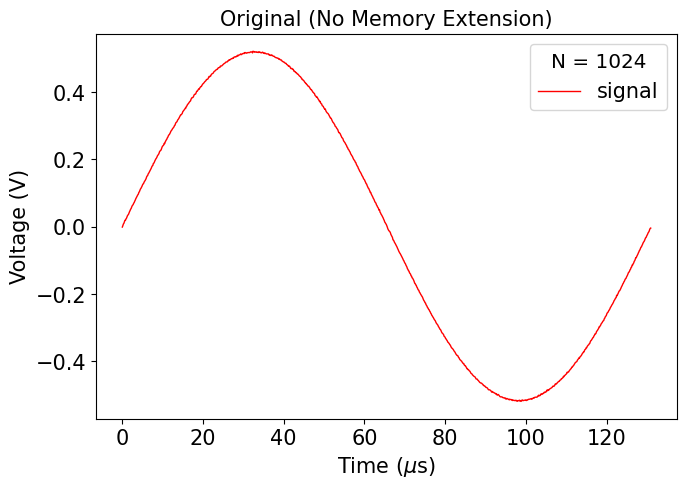
\includegraphics[width=\textwidth]{images/chapter_2/2_li_pid/original.png}
        \caption{}
        \label{fig:ch2_lipid_og}
    \end{subfigure}
    \hspace{.025\linewidth}
    \begin{subfigure}[t]{0.47\linewidth}
        \centering
        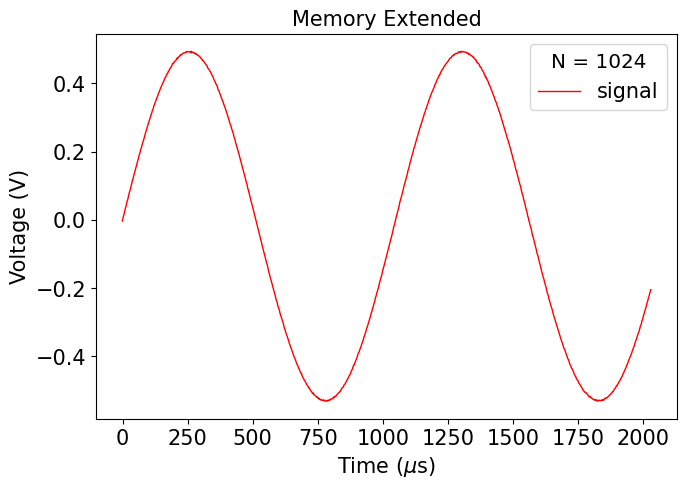
\includegraphics[width=\textwidth]{images/chapter_2/2_li_pid/extended.png}
        \caption{}
        \label{fig:ch2_lipid_ex}
    \end{subfigure}
    \caption{Data exported from the Lock-in+PID oscilloscope application for (a) original and (b) extended allotted system memory space for signal data storage.}
    \label{fig:ch2_lipid}
\end{figure}